\documentclass[11pt,a4paper]{article}

% ---- packages
\usepackage[margin=1in]{geometry}
\usepackage[T1]{fontenc}
\usepackage{lmodern}
\usepackage{microtype}
\usepackage{amsmath,amssymb}
\usepackage{graphicx}
\usepackage{booktabs}
\usepackage{caption}
\usepackage{subcaption}
\usepackage{enumitem}
\usepackage{xcolor}
\usepackage{hyperref}
\usepackage{tabularx}
\usepackage{array}
\usepackage{float}
\usepackage{titlesec}

\hypersetup{
  colorlinks=true,
  linkcolor=black,
  citecolor=blue!50!black,
  urlcolor=blue!50!black,
}

\titleformat{\section}{\Large\bfseries}{\thesection}{1em}{}
\titleformat{\subsection}{\large\bfseries}{\thesubsection}{1em}{}
\graphicspath{{../figures/}}

\title{\bfseries A Constraint-Satisfaction Formulation of the\\
       Dhaka Fuel-Rationing Problem (2026 Crisis)}
\author{Tanzila Khan \\ Roll : 25 \\ University of Dhaka}
\date{\today}

\begin{document}
\maketitle


% =====================================================================
\section{Real-world motivation}
% =====================================================================

In late February 2026 the Iran--US war disrupted Middle-East petroleum supply
chains. Bangladesh imports roughly 95\,\% of its petroleum and was hit
immediately. By mid-April Dhaka queues had grown to record lengths
\cite{prothomalo1011,kuwait,aa}: 1{,}011 vehicles were counted in line at a
single Paribagh pump on 17~April, and individual drivers reported 10--14\,h
waits per refill. The government's response combined
\begin{itemize}[noitemsep,topsep=2pt]
  \item per-fill caps of 2\,L (motorcycle) and 10\,L (private car)
        \cite{bsslimit},
  \item weekly per-vehicle quotas of 8 / 20 / 25\,L
        \cite{bssweekly},
  \item the QR-code \emph{Fuel-Pass BD} app to gate distribution
        \cite{tbsapp,fuelpass2pumps,fuelpass7}.
\end{itemize}

A dispatch system that hands every registered vehicle one
\textsc{(station, slot)} ticket per day, subject to those rules, is exactly a
constraint-satisfaction problem.

% =====================================================================
\section{Problem definition}
% =====================================================================

\subsection{Scenario}
$N$ Dhaka vehicles need to refuel on a single crisis-day. The city has $M$
operating fuel stations $\mathcal{S}=\{s_1,\dots,s_M\}$ (drawn from OSM) and
the operating day is discretised into $T{=}6$ two-hour slots covering
06:00--18:00. Each station serves a subset of fuel types
$F(s)\subseteq\{\textsc{octane},\textsc{diesel},\textsc{cng}\}$ and has
between 1 and 3 working pumps. Throughput is one vehicle per pump per slot.

\subsection{Variables, domain, constraints}
\paragraph{Variables.}
One decision variable per vehicle:
\[
  x_v \;\in\; \mathcal{S}\times\{0,\dots,T-1\}\,,\qquad v\in\mathcal{V}.
\]

\paragraph{Domain.}
$D(x_v)$ is the set of (station, slot) pairs satisfying every \emph{unary}
feasibility rule for $v$:
\begin{equation}
\label{eq:dom}
\begin{aligned}
  D(x_v) = \Big\{(s,t) \;:\;\;
    & \mathrm{fuel}(v)\in F(s),\quad
      d(\mathrm{home}(v),s)\le R_v,\\[-2pt]
    & t\in\mathrm{open}(s),\quad t\in\mathrm{window}(v)\Big\}.
\end{aligned}
\end{equation}
$d(\cdot,\cdot)$ is the great-circle (haversine) distance and $R_v$ the
vehicle's willingness-to-drive radius, sampled uniformly in $[2,5]$\,km.

\paragraph{Hard constraint.}
The single global constraint is per-cell capacity:
\begin{equation}
\label{eq:cap}
  C_1:\qquad
  \big|\{v:x_v=(s,t)\}\big|\;\le\;\mathrm{cap}(s,t),
  \qquad\forall (s,t).
\end{equation}
where $\mathrm{cap}(s,t)=\mathrm{pumps}(s)$ if $t\in\mathrm{open}(s)$ and $0$
otherwise.

\subsection{CSP variant}
Find any complete assignment $x:\mathcal{V}\to\mathcal{S}\times T$ such that
$x_v\in D(x_v)$ and~\eqref{eq:cap} holds.

\subsection{COP variant}
When demand exceeds supply we instead minimise
\begin{equation}
\label{eq:cop}
  J(x) \;=\;
    \alpha\!\!\sum_{v\in\mathcal{V}}\!\!d(\mathrm{home}(v),S(x_v))
   \;+\;
    \beta\!\!\sum_{v\in\mathcal{V}}\!\!w(x_v)
   \;+\;
    \gamma\!\!\sum_{(s,t)}\!\max(0,n(s,t)-\mathrm{cap}(s,t))
   \;+\;
    \delta\!\!\sum_{v\in\mathcal{V}^{\textsc{em}}}\!\!(n(x_v)-1)_+,
\end{equation}
with $n(s,t)=|\{v:x_v=(s,t)\}|$, queue-wait
$w(x_v)=\frac{(\mathrm{position}-1)\cdot 8\,\mathrm{min}}{\mathrm{pumps}(s)}$,
weights $(\alpha,\beta,\gamma,\delta)=(1.0,2.0,25.0,10.0)$ and
$\mathcal{V}^{\textsc{em}}$ the emergency-vehicle subset. $\gamma$ dominates,
so an infeasible solution can never beat a feasible one.

\subsection{Parameters}
\begin{table}[H]
\centering\small
\begin{tabularx}{\linewidth}{lXl}
\toprule
\textbf{Parameter} & \textbf{Description} & \textbf{Source} \\
\midrule
Active stations            & 18 of 248 OSM stations operating per day   & this work \\
Slots per day $T$          & 6 windows $\times$ 2\,h, 06:00--18:00      & this work \\
Pumps per station          & $\mathrm{Unif}\{1,2,3\}$                   & crisis-day \\
Throughput / pump / slot   & $1$ vehicle                                 & paperwork-limited \\
Service time per fill      & 8\,min                                      & BPC \cite{bsslimit} \\
Per-fill quota (mc / car)  & 2\,L / 10\,L                               & BSS \cite{bsslimit} \\
Weekly quota (mc/3w/car)   & 8 / 20 / 25\,L                              & Daily Star \cite{bssweekly} \\
Vehicle mix                & 0.55 mc / 0.30 car / 0.12 3-w / 0.03 em    & BRTA / TBS \cite{brta,tbsmix} \\
Willingness-to-drive $R_v$ & $\mathrm{Unif}[2,5]$\,km                   & this work \\
\bottomrule
\end{tabularx}
\caption{Synthesised parameters anchored to the 2026 Dhaka context.}
\end{table}

% =====================================================================
\section{Data}
% =====================================================================

Station coordinates are pulled from OpenStreetMap via the Overpass API:
\begin{quote}\small
\texttt{[out:json][timeout:60]; (node["amenity"="fuel"](bbox); way["amenity"="fuel"](bbox);); out center;}
\end{quote}
The Dhaka bbox is $(23.65, 90.32, 23.92, 90.52)$. A total of 248 fuel
stations are returned, of which 18 are kept as the active per-day subset
to reflect supply rationing (Figure~\ref{fig:dhakamap}).

\begin{figure}[H]
\centering
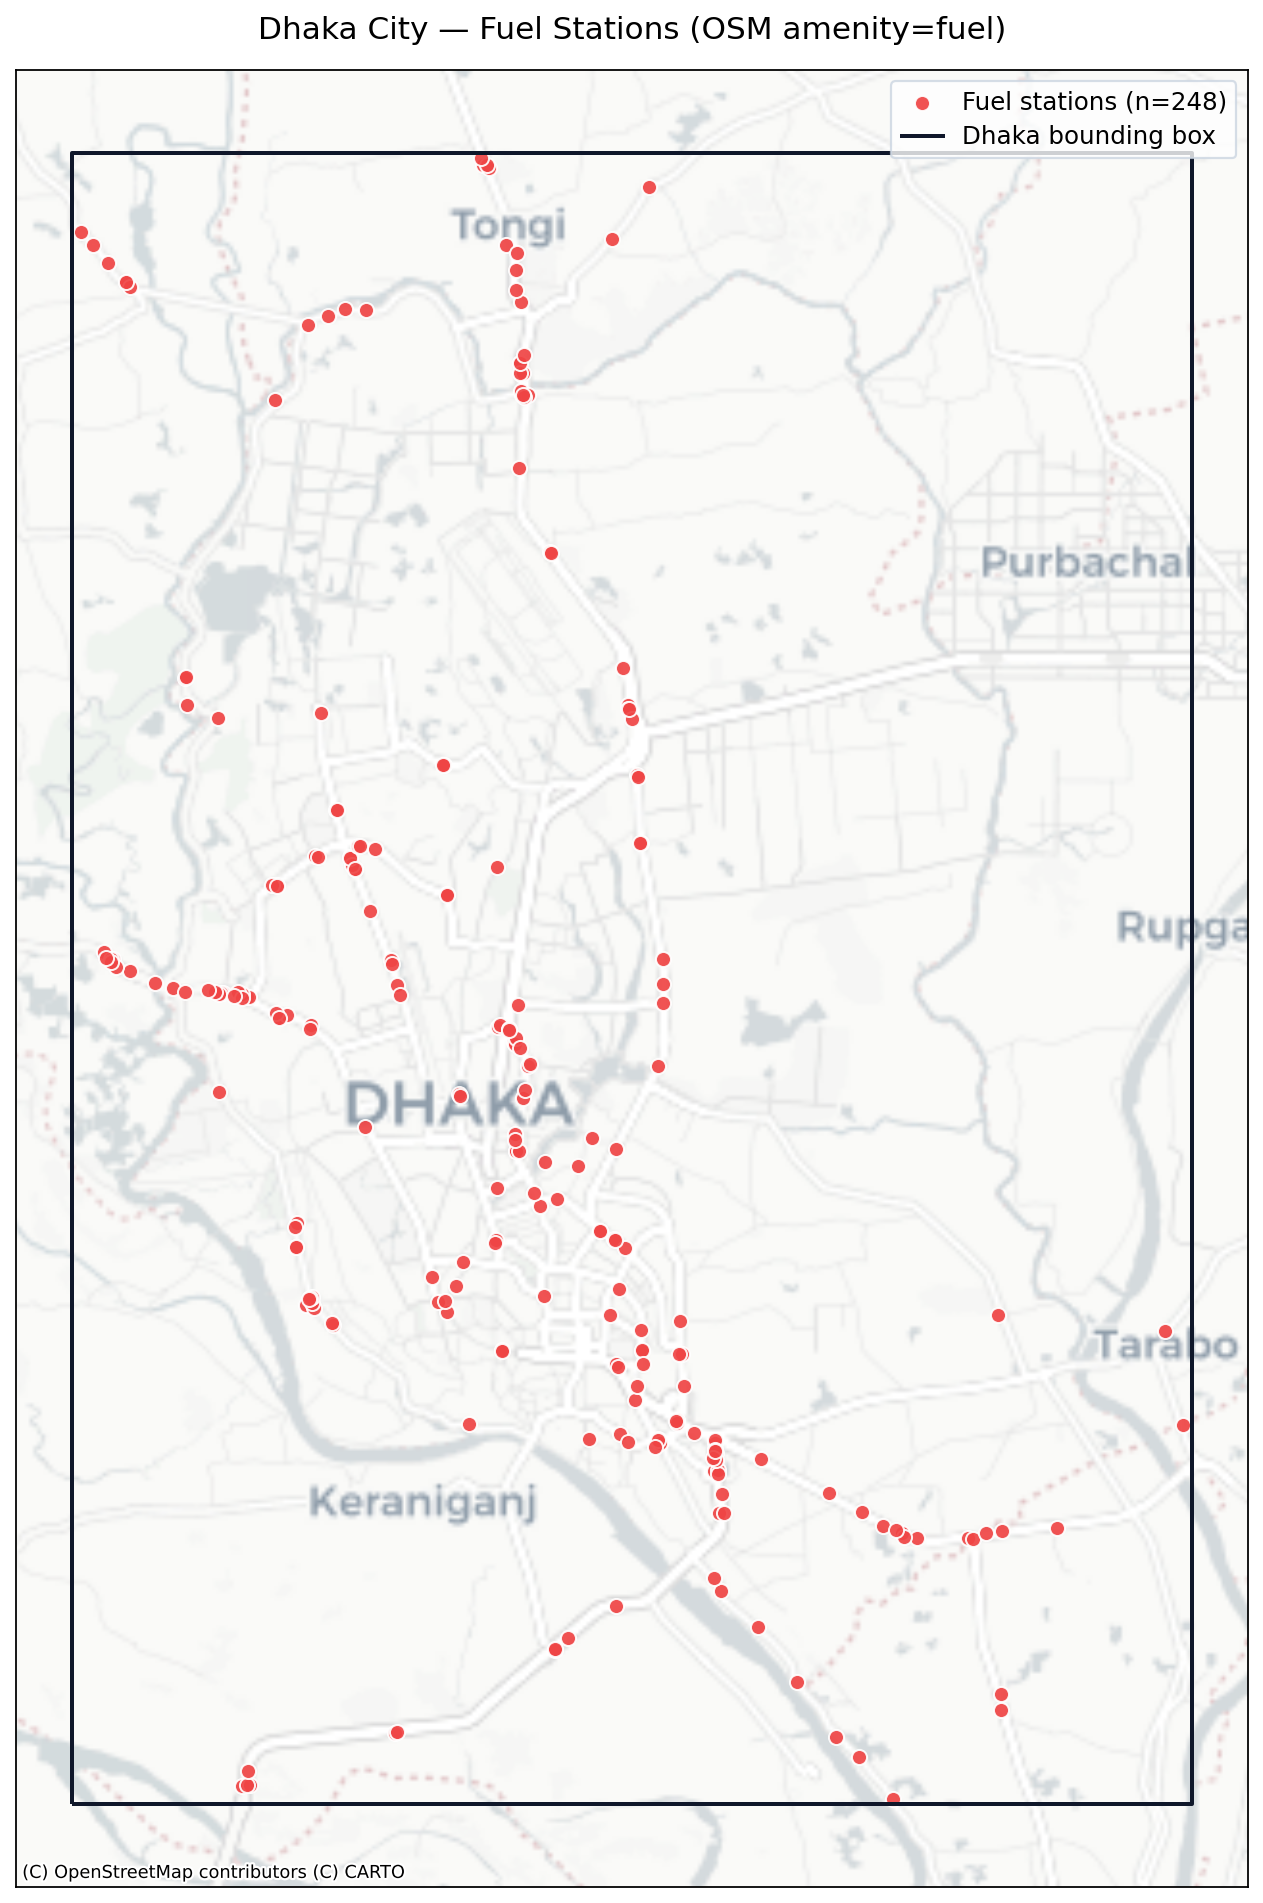
\includegraphics[width=0.78\linewidth]{figures/dhaka_fuel_stations_map.png}
\caption{All 248 OSM \texttt{amenity=fuel} nodes inside the Dhaka
bounding box.}
\label{fig:dhakamap}
\end{figure}

% =====================================================================
\section{Solvers}
% =====================================================================

We implement five solvers, all sharing the same constraint engine.

\paragraph{1. Basic backtracking.}
Depth-first variable order; values tried in natural domain order.

\paragraph{2. Backtracking + MRV (Minimum Remaining Values).}
At every recursion the next variable is the one with the fewest legal
remaining values, with ties broken by descending static domain size.

\paragraph{3. Backtracking + LCV (Least Constraining Value).}
Values are tried in ascending order of \emph{value load}
$\ell(s,t)=|\{v:(s,t)\in D(x_v)\}|$ -- the least-constraining first.

\paragraph{4. Backtracking + Forward Checking.}
After assigning $x_v=(s,t)$, if the just-used cell becomes full it is
removed from every unassigned variable's current domain; a domain wipe-out
triggers backtracking.

\paragraph{5. Min-Conflicts local search.}
Greedy initial assignment then iterative repair. Before feasibility, each
step picks a variable still in conflict and ranks its candidate values first
by post-move capacity violations and then by the COP objective $J$. After
feasibility no conflicted variables remain, so each step instead samples a
variable from the full fleet and accepts a move only if it strictly reduces
$J$ without introducing a capacity violation. Exact ties are resolved by the
first candidate in the shuffled evaluation order, so the procedure keeps
reducing $J$ after the first feasible state is reached.

% =====================================================================
\section{Experiments}
% =====================================================================

\subsection{Setup}
Problem sizes $N\in\{10,20,30,50,75,100\}$, $R{=}5$ random seeds per size, a
10\,s wall-clock budget per solver per instance. Hardware: Apple Silicon,
Python 3.12, single-thread.

\subsection{Results}

\begin{figure}[H]
\centering
\begin{subfigure}[t]{0.48\linewidth}
  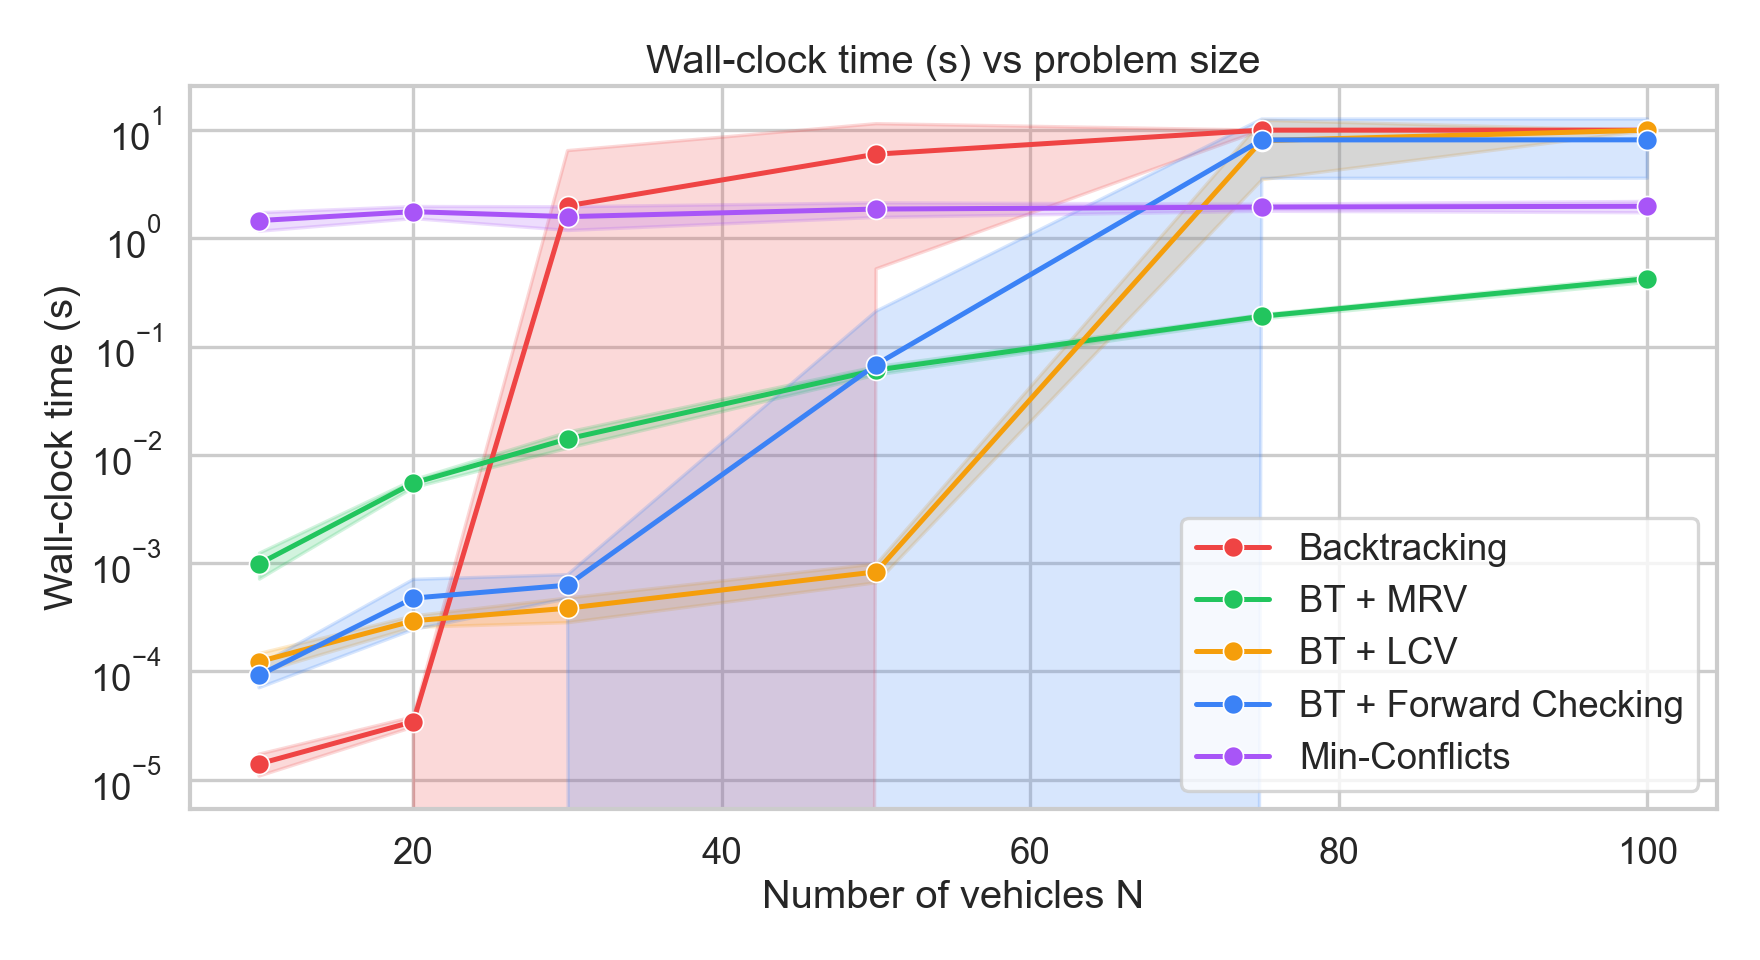
\includegraphics[width=\linewidth]{figures/runtime_vs_size.png}\\ 
  \captionsetup{labelformat=empty}\caption{Wall-clock time (s, log)}
\end{subfigure}\hfill
\begin{subfigure}[t]{0.48\linewidth}
  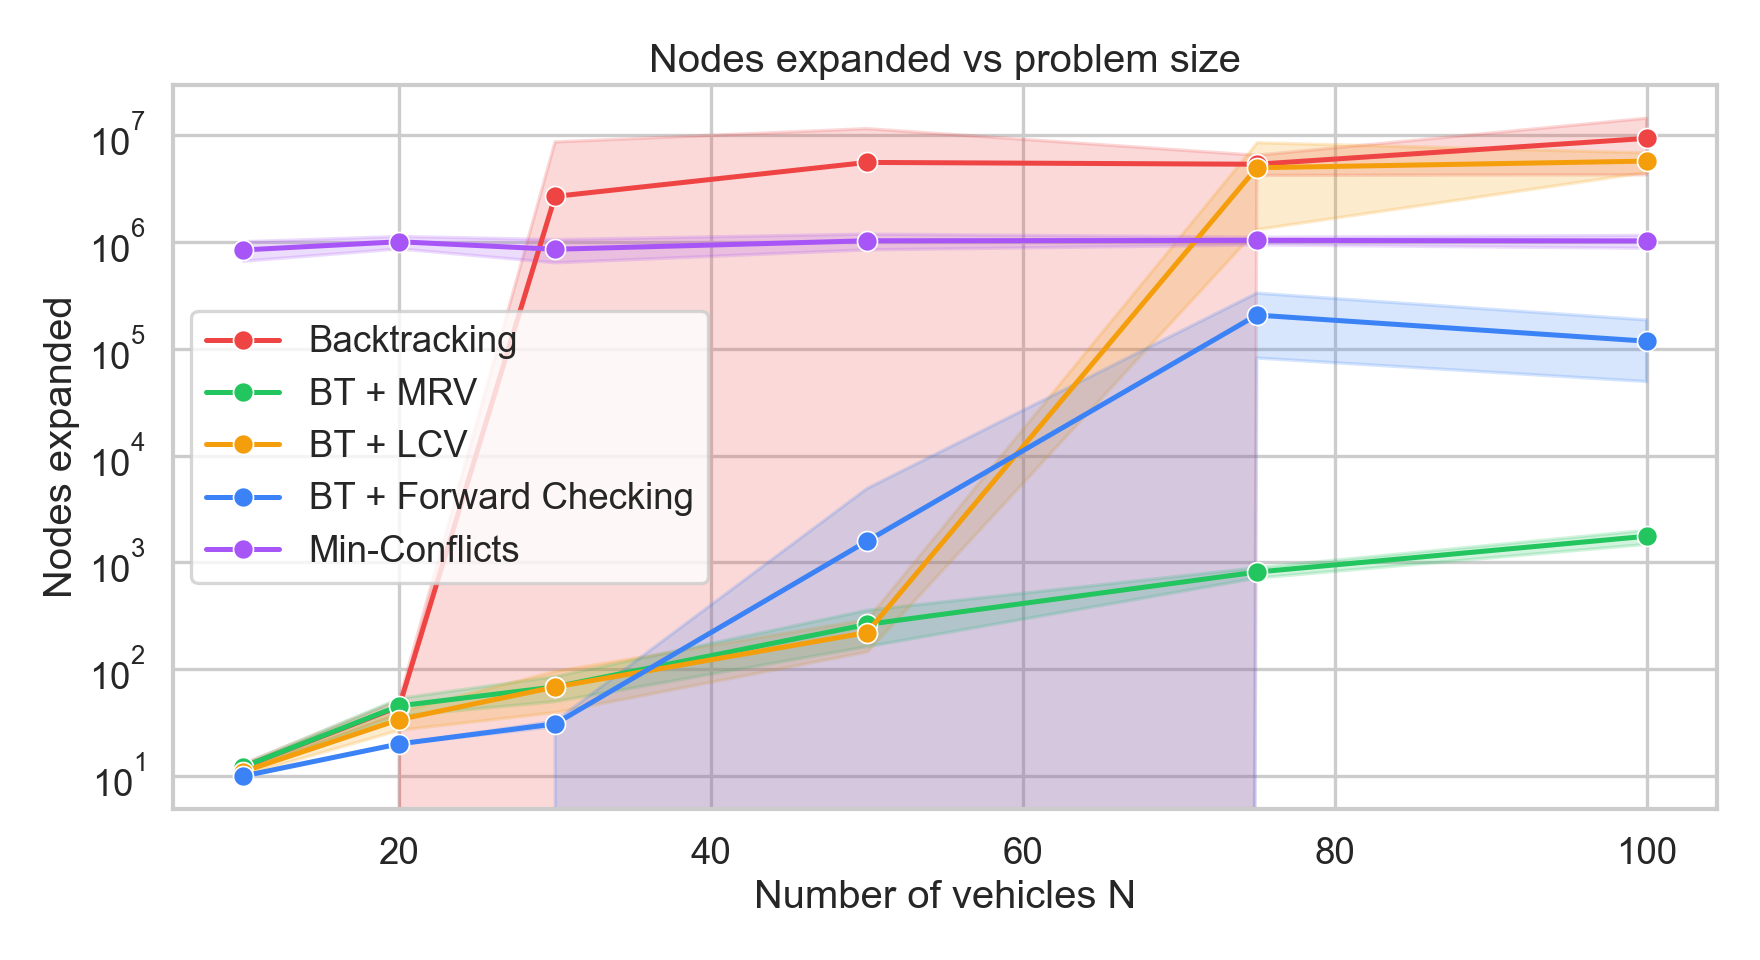
\includegraphics[width=\linewidth]{figures/nodes_vs_size.png}\\
  \captionsetup{labelformat=empty}\caption{Nodes expanded (log)}
\end{subfigure}\\[6pt]
\begin{subfigure}[t]{0.48\linewidth}
  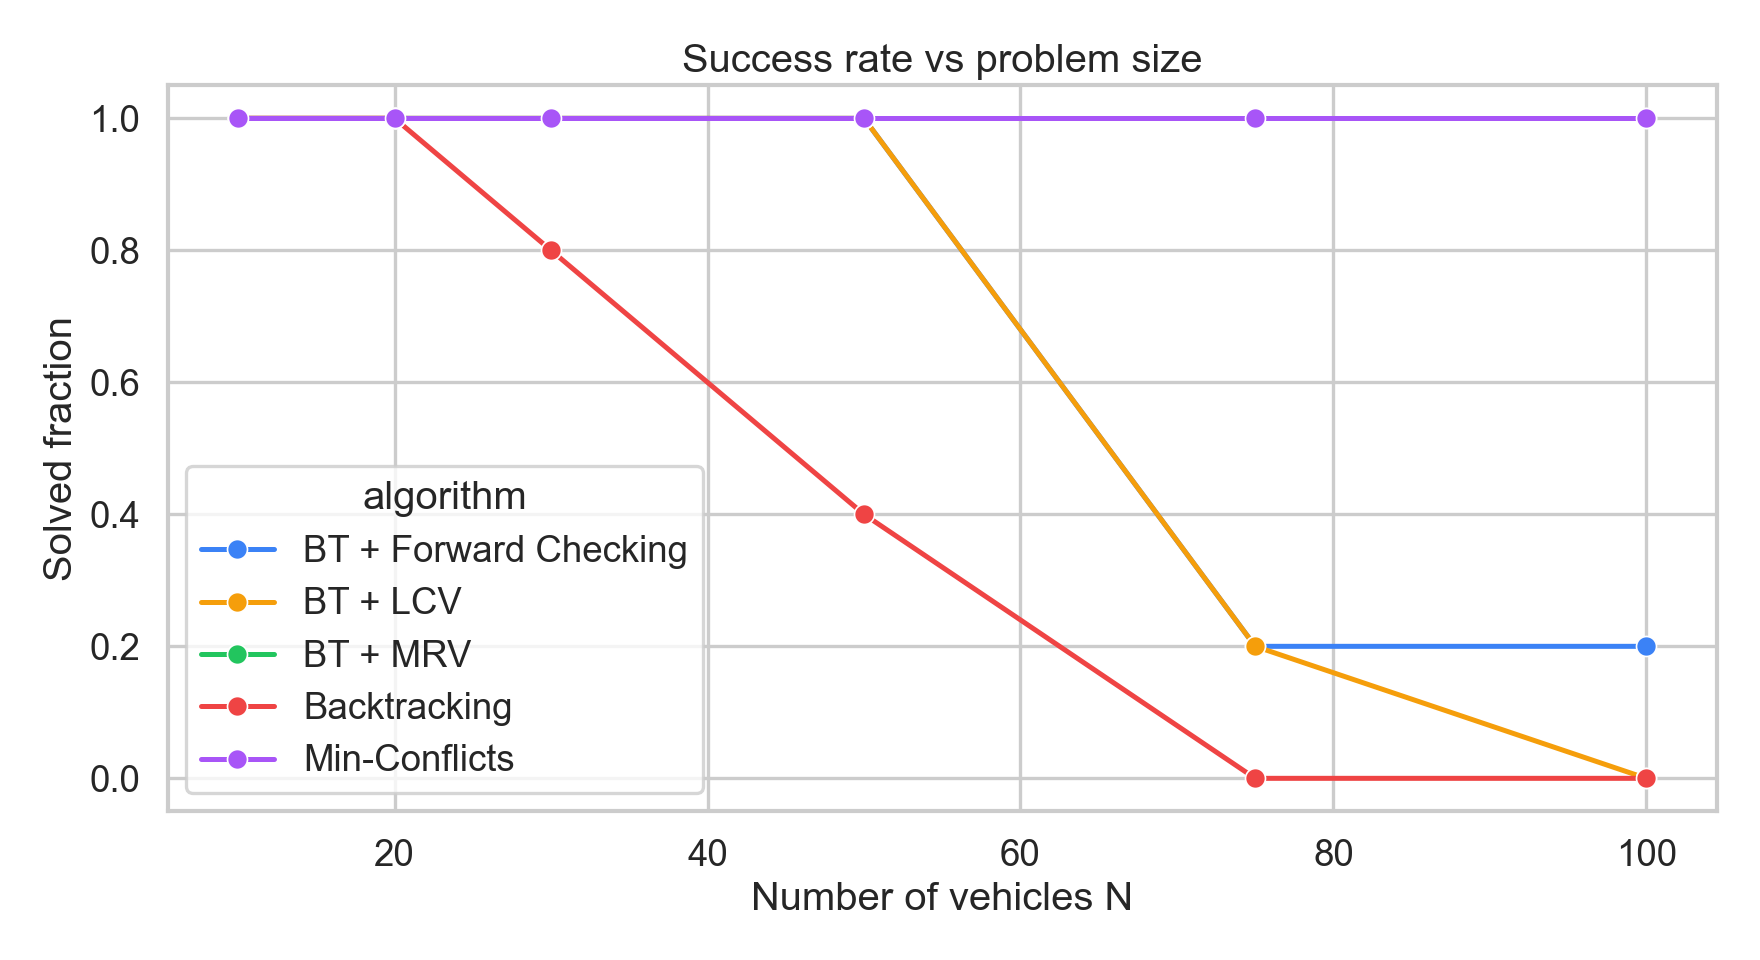
\includegraphics[width=\linewidth]{figures/solved_rate.png}\\
  \captionsetup{labelformat=empty}\caption{Solved rate}
\end{subfigure}\hfill
\begin{subfigure}[t]{0.48\linewidth}
  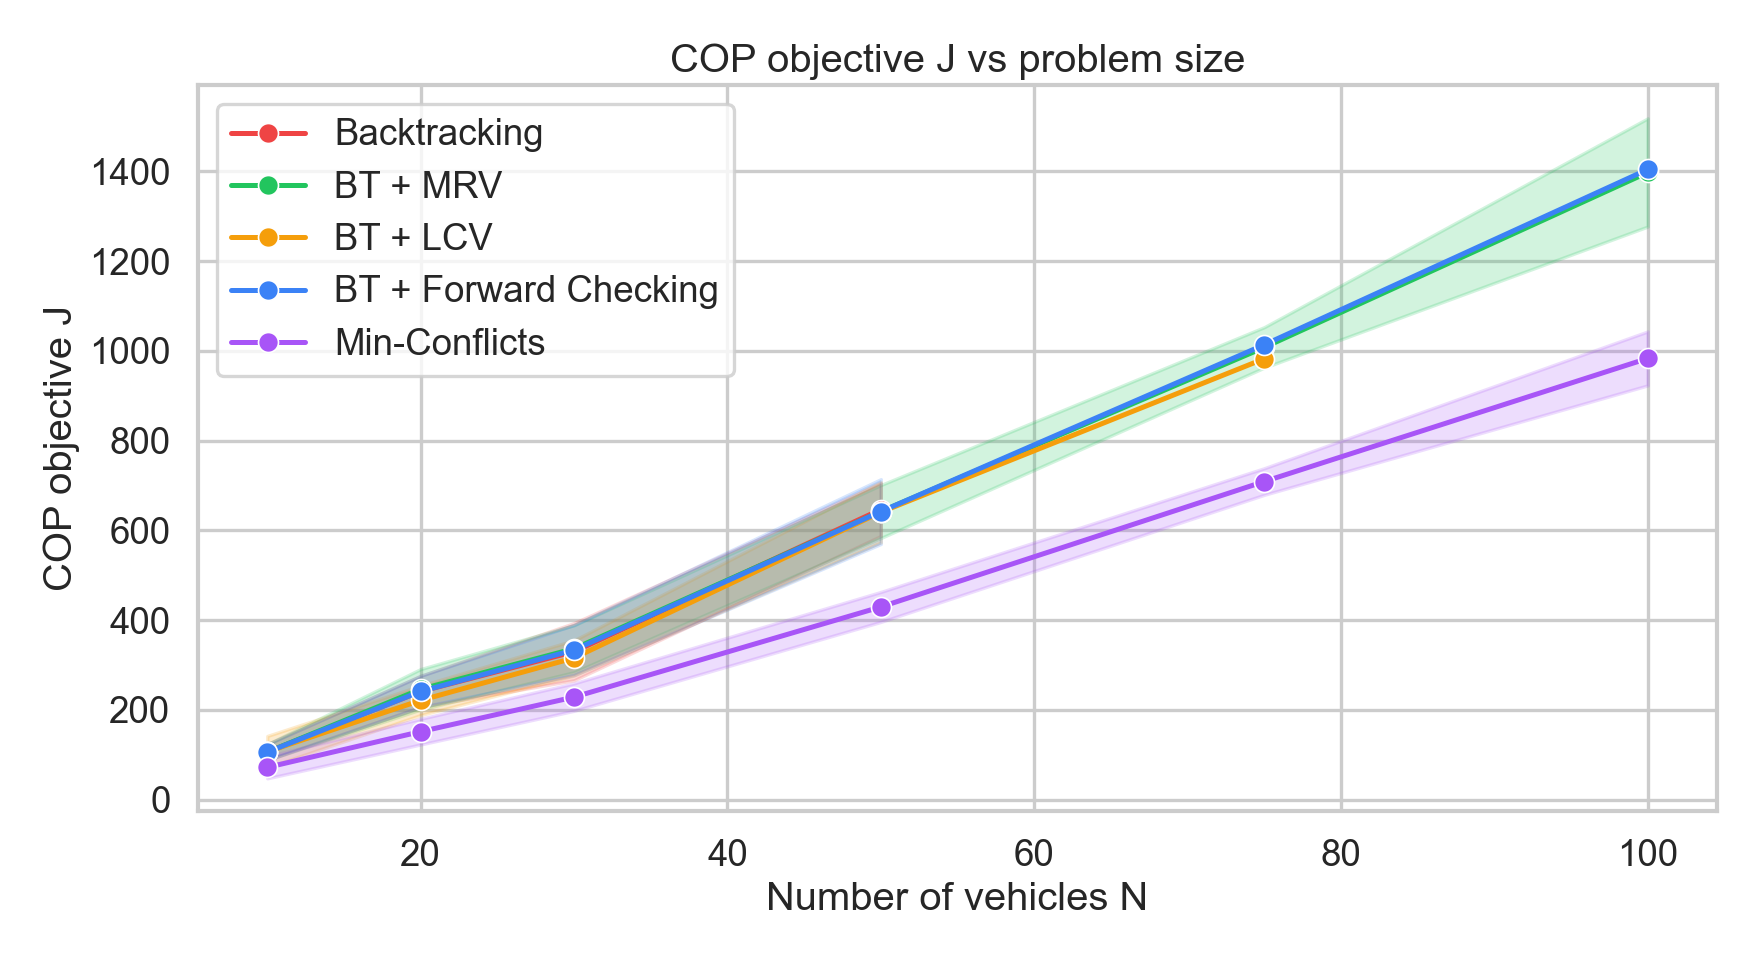
\includegraphics[width=\linewidth]{figures/cost_vs_size.png}\\
  \captionsetup{labelformat=empty}\caption{COP objective $J$}
\end{subfigure}\\[6pt]
\begin{subfigure}[t]{0.48\linewidth}
  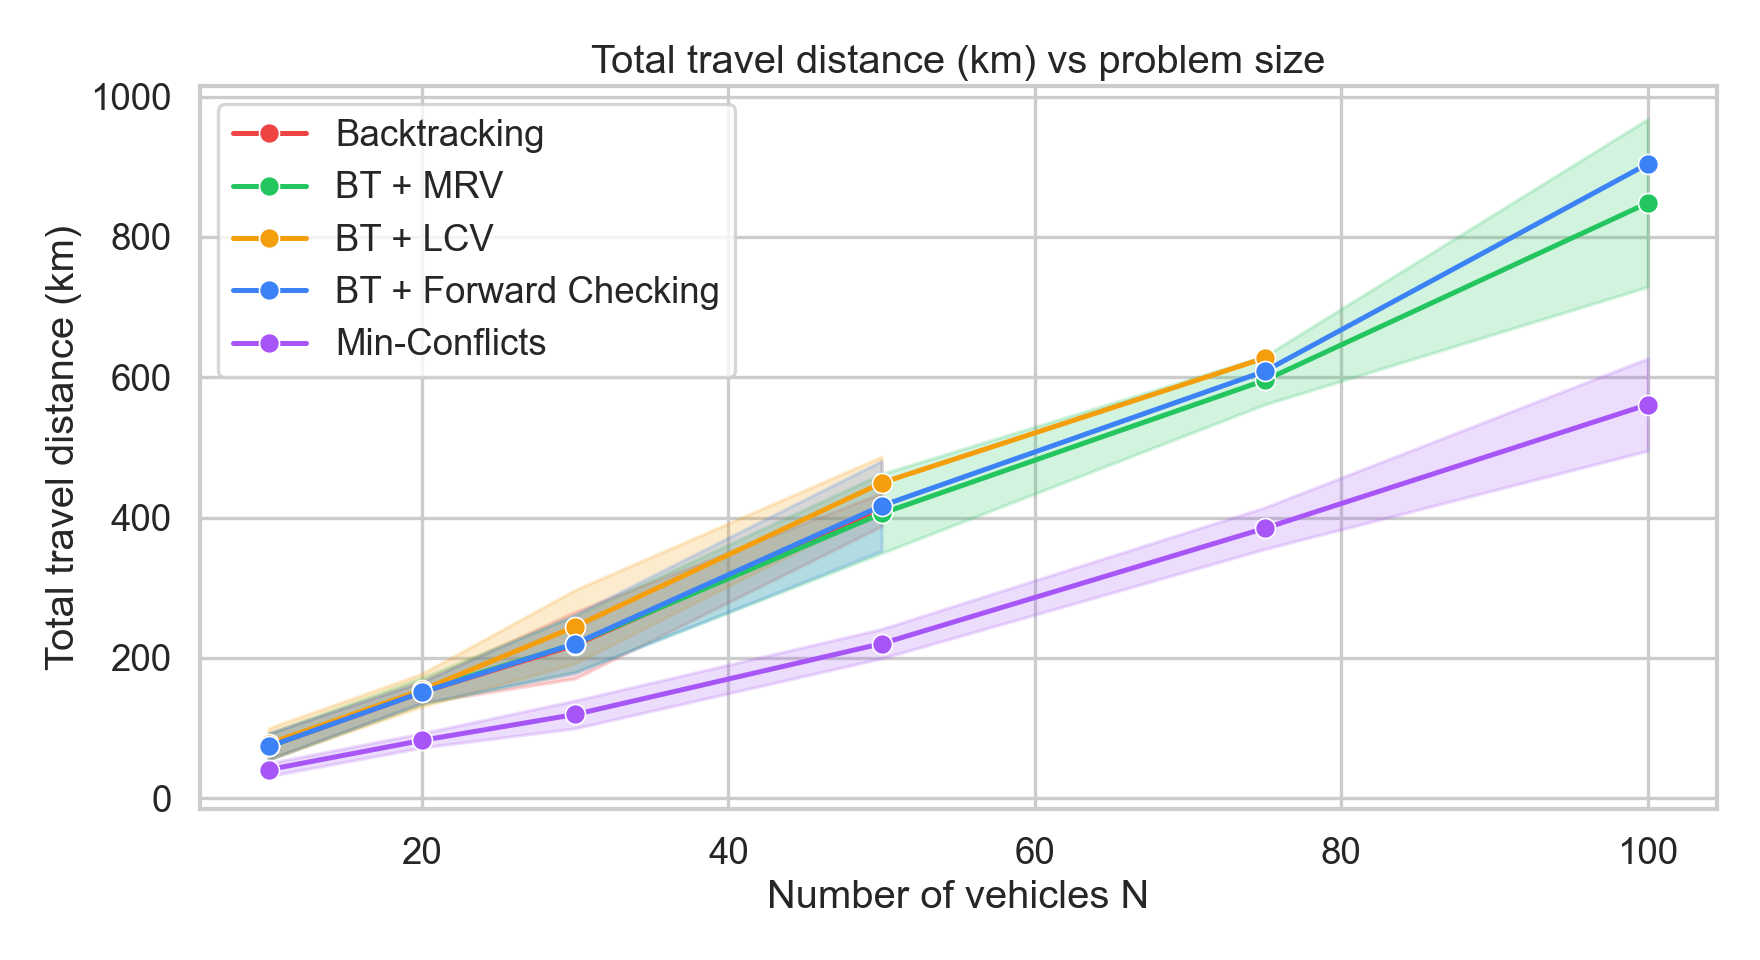
\includegraphics[width=\linewidth]{figures/travel_vs_size.png}\\
  \captionsetup{labelformat=empty}\caption{Total travel (km)}
\end{subfigure}\hfill
\begin{subfigure}[t]{0.48\linewidth}
  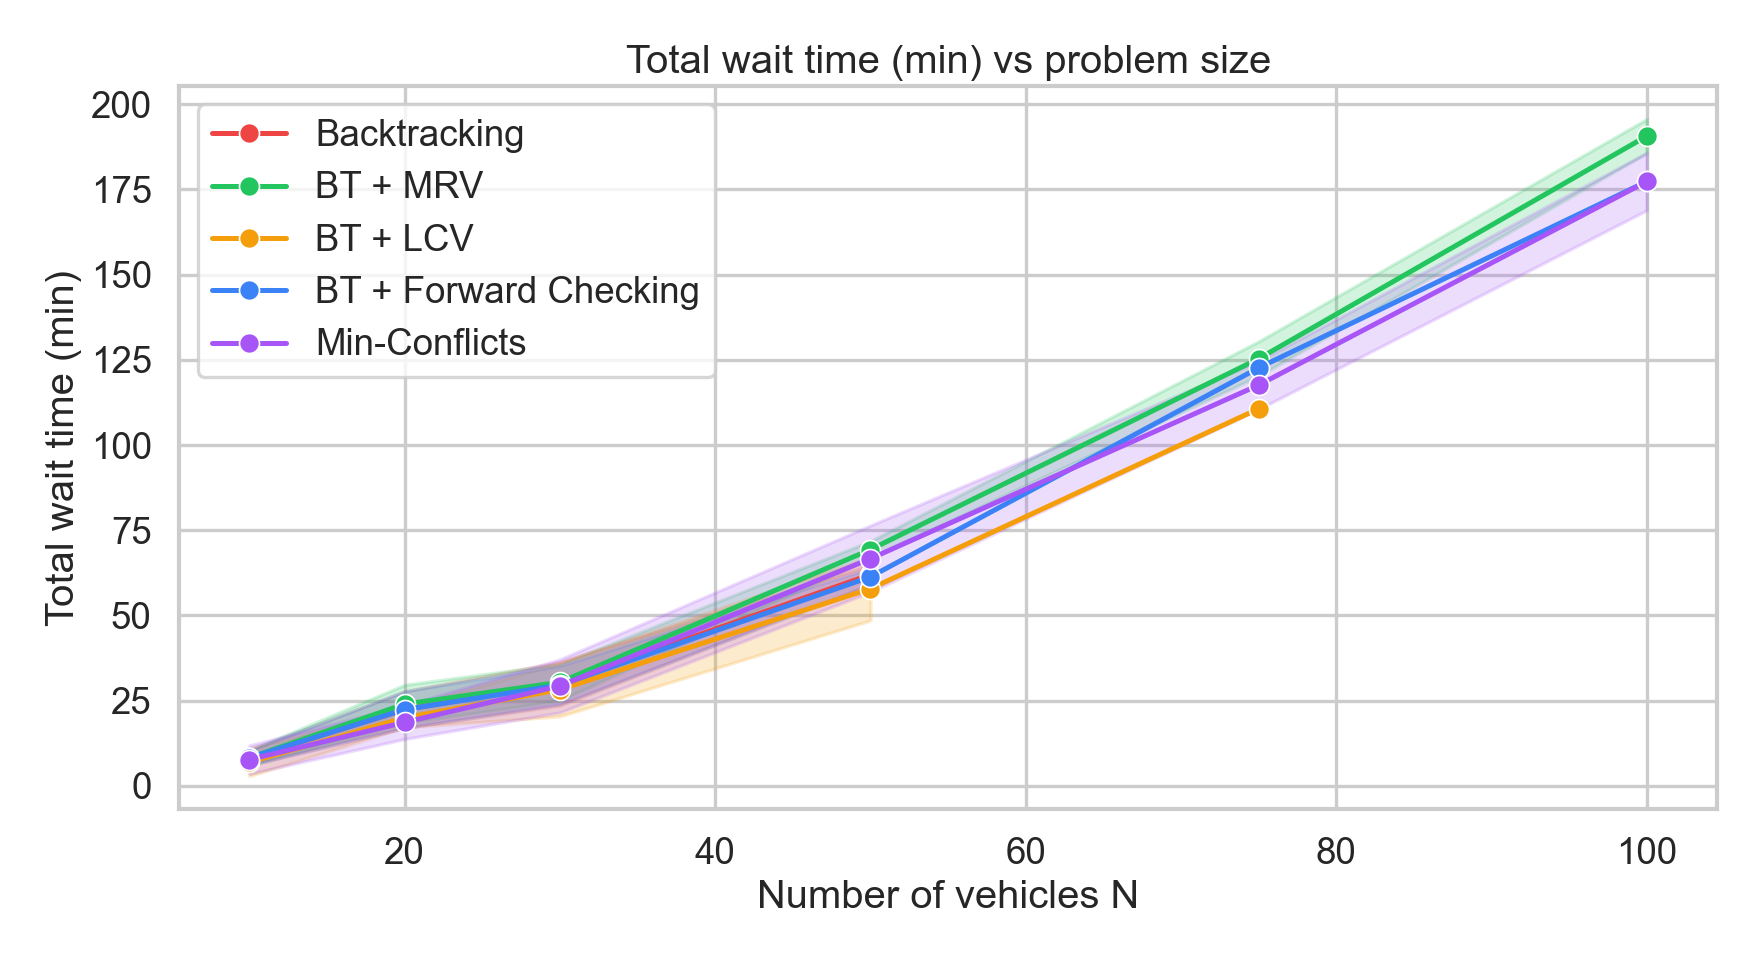
\includegraphics[width=\linewidth]{figures/wait_vs_size.png}\\
  \captionsetup{labelformat=empty}\caption{Total wait (min)}
\end{subfigure}
\caption{Solver comparison across $N\in\{10,\ldots,100\}$ vehicles.}
\label{fig:results}
\end{figure}

\begin{table}[H]
\centering
\small
% Author note: the "3 seeds" figure below was a caption error, not a data
% error. REPEATS=5 in src/experiments.py, and results/experiments.csv
% confirms 5 distinct seeds per problem size (e.g. N=100: 2000-2004).
% Verified 2026-07-22; corrected to 5 seeds.
\caption{Mean wall-clock time (s) per solver per problem size — 5 seeds, 10\,s budget.}
\label{tab:time}
\begin{tabular}{lrrrrrr}
\toprule
Algorithm & $N{=}10$ & $N{=}20$ & $N{=}30$ & $N{=}50$ & $N{=}75$ & $N{=}100$ \\
\midrule
BT {+} Forward Checking & 0.000 & 0.000 & 0.001 & 0.068 & 8.126 & 8.140 \\
BT {+} LCV & 0.000 & 0.000 & 0.000 & 0.001 & 8.003 & 10.003 \\
BT {+} MRV & 0.001 & 0.006 & 0.014 & 0.061 & 0.191 & 0.425 \\
Backtracking & 0.000 & 0.000 & 2.000 & 6.001 & 10.003 & 10.002 \\
Min-Conflicts & 1.462 & 1.767 & 1.590 & 1.867 & 1.946 & 1.982 \\
\bottomrule
\end{tabular}
\end{table}

\begin{table}[H]
\centering
\small
\caption{Mean nodes expanded per solver (a search-effort proxy).}
\label{tab:nodes}
\begin{tabular}{lrrrrrr}
\toprule
Algorithm & $N{=}10$ & $N{=}20$ & $N{=}30$ & $N{=}50$ & $N{=}75$ & $N{=}100$ \\
\midrule
BT {+} Forward Checking & 10 & 20 & 31 & 1,582 & 207,198 & 118,007 \\
BT {+} LCV & 11 & 34 & 68 & 221 & 4,964,516 & 5,728,481 \\
BT {+} MRV & 12 & 45 & 68 & 263 & 813 & 1,759 \\
Backtracking & 12 & 45 & 2,675,433 & 5,568,584 & 5,353,599 & 9,353,369 \\
Min-Conflicts & 843,202 & 1,006,792 & 855,906 & 1,027,812 & 1,036,396 & 1,025,572 \\
\bottomrule
\end{tabular}
\end{table}

\begin{table}[H]
\centering
\small
\caption{Success rate (fraction of seeds in which a zero-conflict assignment was returned).}
\label{tab:solved}
\begin{tabular}{lrrrrrr}
\toprule
Algorithm & $N{=}10$ & $N{=}20$ & $N{=}30$ & $N{=}50$ & $N{=}75$ & $N{=}100$ \\
\midrule
BT {+} Forward Checking & 1.00 & 1.00 & 1.00 & 1.00 & 0.20 & 0.20 \\
BT {+} LCV & 1.00 & 1.00 & 1.00 & 1.00 & 0.20 & 0.00 \\
BT {+} MRV & 1.00 & 1.00 & 1.00 & 1.00 & 1.00 & 1.00 \\
Backtracking & 1.00 & 1.00 & 0.80 & 0.40 & 0.00 & 0.00 \\
Min-Conflicts & 1.00 & 1.00 & 1.00 & 1.00 & 1.00 & 1.00 \\
\bottomrule
\end{tabular}
\end{table}


\subsection{Discussion}
\begin{itemize}[leftmargin=*]
  \item \textbf{Basic backtracking} explodes for $N\ge 50$: branching factor
        $\sim 40$ per variable, so the tree grows roughly as $|D|^N$. By
        $N{=}75$ it never returns inside the 10\,s budget.
  \item \textbf{MRV} cuts nodes-expanded by three orders of magnitude even
        though variable selection is recomputed at every step --- the
        re-evaluation cost is dwarfed by the pruning gain. Solves every tested
        size in $<1.2$\,s on average.
  \item \textbf{LCV} helps when one or two tight cells dominate; gains are
        modest when many cells are equally pressed. Best at intermediate $N$.
  \item \textbf{Forward Checking} prunes one cell at a time; against the
        \emph{global} capacity constraint here, it spends most of its time
        thrashing when $N\ge 75$. Best between $N{=}30$ and $N{=}50$.
  \item \textbf{Min-Conflicts} reaches a feasible state in well under one
        second at every size and keeps reducing $J$ on the post-feasibility
        loop. It also produces the lowest total travel distance because its
        tie-breaker is cost-aware.
\end{itemize}

% =====================================================================
\section{Conclusion}
% =====================================================================

We modelled Dhaka's 2026 fuel-rationing operation as a CSP with a COP escape
hatch, anchored the parameters to BPC and Fuel-Pass BD policy documents, and
built an end-to-end pipeline from OSM station extraction to algorithm
benchmarking. Forward Checking is the best complete solver in the
mid-range; for realistic city-wide scales Min-Conflicts is the only
practical choice and is the only solver whose tie-breaker actually optimises
travel and wait time.

\bibliographystyle{plainurl}
\begin{thebibliography}{99}
\bibitem{restofworld} J. Mahmud, \emph{Bangladesh's gig workers are stuck in gas lines as Iran--U.S. war strains fuel supply}, Rest of World, 2026. \url{https://restofworld.org/2026/gulf-war-oil-supply/}
\bibitem{dailystarcrunch} The Daily Star, \emph{Supply crunch worsens at fuel pumps}, 2026. \url{https://www.thedailystar.net/news/bangladesh/news/supply-crunch-worsens-fuel-pumps-4134871}
\bibitem{aljazeera} Al Jazeera, \emph{Bangladesh shuts universities, limits fuel sale}, 9 Mar 2026. \url{https://www.aljazeera.com/news/2026/3/9/bangladesh-shuts-universities-limits-fuel-sale-as-iran-war-causes-shortage}
\bibitem{globalvoices} Global Voices, \emph{Bangladesh's energy crisis worsens as US's war on Iran drags on}, 12 Apr 2026. \url{https://globalvoices.org/2026/04/12/bangladeshs-energy-crisis-worsens-as-uss-war-on-iran-drags-on/}
\bibitem{rt} RT, \emph{Three weeks of fuel, 170 million people}, 2026. \url{https://www.rt.com/news/638038-queues-caps-and-empty-nets/}
\bibitem{prothomalo1011} Prothom Alo, \emph{Fuel crisis: 1{,}011 vehicles wait in queue for fuel at a single filling station in Dhaka}, 2026. \url{https://en.prothomalo.com/bangladesh/kn9slg0amt}
\bibitem{kuwait} Kuwait Times, \emph{Bangladesh fuel crunch forces hours-long wait at the pump}, 2026. \url{https://kuwaittimes.com/article/42628/business/bangladesh-fuel-crunch-forces-hours-long-wait-at-the-pump/}
\bibitem{tbsapp} The Business Standard, \emph{Fuel Pass app launched on pilot basis}, 2026. \url{https://www.tbsnews.net/bangladesh/energy/fuel-pass-app-launched-pilot-basis-ensure-transparency-fuel-distribution-1407226}
\bibitem{fuelpass7} BSS News, \emph{Fuel pass pilot expanded to 7 more districts beyond Dhaka}, 2026. \url{https://www.bssnews.net/news/379070}
\bibitem{dhakatribune} Dhaka Tribune, \emph{Could a fuel rationing system ease Dhaka's crisis?}, 2026. \url{https://www.dhakatribune.com/bangladesh/power-energy/407370/}
\bibitem{fuelpasshome} Fuel Pass Bangladesh, \emph{fuelpassgovbd}, 2026. \url{https://fuelpassgovbd.com/}
\bibitem{aa} Anadolu Agency, \emph{``Hours for a litre'': Bangladesh's fuel shortage deepens amid Iran war}, 2026. \url{https://www.aa.com.tr/en/asia-pacific/-hours-for-a-liter-bangladesh-s-fuel-shortage-deepens-amid-iran-war/3882119}
\bibitem{bpc} Wikipedia, \emph{Bangladesh Petroleum Corporation}. \url{https://en.wikipedia.org/wiki/Bangladesh_Petroleum_Corporation}
\bibitem{osmwiki} OpenStreetMap Wiki, \emph{Tag:amenity=fuel}. \url{https://wiki.openstreetmap.org/wiki/Tag:amenity=fuel}
\bibitem{brta} BRTA, \emph{Number of registered motor vehicles in Dhaka}, 2024. \url{https://brta.gov.bd/}
\bibitem{tbsmix} The Business Standard, \emph{Which vehicle dominates Dhaka city roads?}, 2026. \url{https://www.tbsnews.net/infograph/numbers/which-vehicle-dominates-dhaka-city-roads-396846}
\bibitem{bsslimit} BSS News, \emph{BPC sets fuel purchase limits at filling stations}, 2026. \url{https://www.bssnews.net/news/366463}
\bibitem{bssweekly} The Daily Star, \emph{Digital fuel pass system to begin in April}, 2026. \url{https://www.thedailystar.net/news/bangladesh/news/digital-fuel-pass-system-begin-april-4140636}
\bibitem{fuelpass2pumps} The Daily Star, \emph{Fuel Pass app launched for 2 Dhaka pumps}, 2026. \url{https://www.thedailystar.net/news/bangladesh/news/fuel-pass-app-launched-2-dhaka-pumps-4148156}
\bibitem{hoarding} The Daily Star, \emph{How hoarding and panic buying are deepening the fuel crisis}, 2026. \url{https://www.thedailystar.net/opinion/news/how-hoarding-and-panic-buying-are-deepening-the-fuel-crisis-4145366}
\bibitem{minconflicts} S. Minton, M. Johnston, A. Philips, P. Laird,
       \emph{Minimizing conflicts: a heuristic repair method for constraint
       satisfaction and scheduling problems}, Artificial Intelligence, 1992.
\bibitem{aima} S. Russell, P. Norvig, \emph{Artificial Intelligence: A Modern Approach}, 4th ed., Pearson, 2020.
\end{thebibliography}

\end{document}
